\section{Experiments and Discussion}\label{sec:experiments}

The performance of our collaborative preference model with the BALD active learning strategy
is evaluated in a series of experiments with simulated and real-world data.
The analyzed datasets include a) synthetic data generated from the probabilistic model assumed by
the proposed multi-user method (Synthetic), b) a collection of user preferences on different movies (MovieLens),
c) the number of votes obtained by different political parties in the 2010 UK general election (Election), 
d) preferences of users about different types of sushi (Sushi), and finally, e)
information regarding the concentration of heavy metals in the Swiss Jura region (Jura).
Section 6 in the supplementary material contains a detailed description of these datasets.

\subsection{Comparison with other multi-user methods}

\paragraph{Alternative models.} Two versions of the proposed collaborative preference (CP) model are used.
The first version (CPU) takes into account the available user features, as described in Section \ref{sec:model}. The second version (CP) ignores these features by
replacing $\mathbf{K}_\text{users}$ in (\ref{eq:priorW}) with the identity matrix.
The first multi-user method we compare to is the approach of Birlitiu et al. (BI) \cite{birlutiu2009}.
This method does not use user features, and captures similarities between users with a hierarchical GP model. In particular,
a common GP prior is assumed for the preference function of each user; using this prior the model learns 
the full GP posterior for each user.
The second multi-user method is the technique of Bonilla et al. (BO) \cite{Bonilla2010}.
In this model there exists one high-dimensional function which depends on both
the features of the two items to be compared and on the features of the user who makes the comparison. Relationships between users' behaviors are captured only via the user features.
We implement BO and BI using the preference kernel and EP for approximate inference\footnote{Although
this is not the same as the original implementations (sampling-based for BI, Laplace approximation for BO), 
the preference kernel and EP are likely to augment the performance of these algorithms, 
and provides the fairest comparison of the underlying models.}.
The computational costs of BO and BI are rather high; BO has cubic complexity in the \emph{total} number of observations i.e. $\mathcal{O}((\sum_{u=1}^UM_u)^3)$, 
our model (CPU) has a significantly lower cost of $\mathcal{O}(D(U^3+P^3))$ (before further speed-up from FITC). 
BI does not include 
user features, but learns $U$ GPs, so has complexity $\mathcal{O}(UP^3)$; the equivalent version of our model
(CP) has cost $\mathcal{O}(NP+DP^3)$, which is lower because $D<<U$.
More details about BI and BO are given in sections 7 and 8 of the supplementary material.
Finally, we consider a single user approach (SU) which fits a different GP classifier independently to the data of each user.

\paragraph{Experimental procedure.} Due to the high computational cost of BI and BO, to compare to these methods we must subsample the datasets, keeping only 100 users.
The available data were split randomly into training and test sets of item pairs,
where the training sets contain 20 pairs per user in Sushi, MovieLens and Election, 15 pairs in Jura and
30 in Synthetic. This was repeated 25 times to obtain statistically meaningful results.
In CPU and CP, we selected the number of latent functions $D$ to be $20$ (see Table \ref{tab:small}).
In general, the proposed models, CPU and CP, are robust to over-fitting and over-estimation of
$D$ does not harm predictive performance. Note that the Synthetic dataset is generated
using $D=5$ and CPU and CP still obtain very good results using $D = 20$.
This automatic pruning of unnecessary degrees of freedom seems to be common
in methods based on variational Bayes \cite{MacKay2001}.
We selected the kernel lengthscales to be equal to
the median distance between feature vectors. This leads to good empirical performance
for most methods. An exception is BO, where the kernel hyperparameters
are tuned to some held-out data using automatic relevance determination.
In our model, we can also estimate the kernel
lengthscales by maximizing the EP approximation of the model evidence,
as illustrated in Section 9 of the supplementary material. This alternative approach can be used
when it is necessary to fine tune the lengthscale parameters to the data. In CPU we use $U_0 = 25$ pseudo inputs for approximating $\mathbf{K}_\text{users}$.
These pseudo inputs are selected randomly from the set of available data points.
Similarly, in CP and CPU, we use $P_0 = 25$ pseudo inputs for approximating $\mathbf{K}_\text{items}$,
except in the Jura and Election datasets (which contain fewer items) where we use $P_0 = 15$.
The results obtained are not sensitive to the number of pseudo inputs used, as long as
the number is not excessively low.

%\renewcommand{\arraystretch}{0.9}
\newcommand{\ic}{\hspace{0.25cm}}
\begin{table}
\begin{minipage}[b]{0.47\linewidth}
\centering
\caption{Average test error with 100 users.}
\resizebox{0.9 \linewidth}{!}{
\begin{tabular}{@{\ic}l@{\ic}c@{\ic}c@{\ic}c@{\ic}c@{\ic}c@{\ic}c@{\ic}}
\hline
\textbf{Dataset} &\textbf{CPU}&\textbf{CP}&\textbf{BI}&\textbf{BO}&\textbf{SU}\\
\hline
Synthetic&0.162&0.180&0.175&\bf{0.157}&0.226\\
%Synthetic2&0.120&0.128&0.127&\bf{0.113}&0.152\\
Sushi&0.171&0.163&\bf{0.160}&0.266&0.187\\
MovieLens&0.182&\bf{0.166}&0.168&0.302&0.217\\
Election&0.199&0.123&\bf{0.077}&0.401&0.300\\
Jura&0.159&\bf{0.153}&\bf{0.153}&0.254&0.181\\
\hline
\end{tabular} \label{tab:errorSmallDatasets}
}
\end{minipage}
\begin{minipage}[b]{0.53\linewidth}
\centering
\caption{Training times (s) with 100 users.}
\resizebox{0.9 \linewidth}{!}{
\begin{tabular}{@{\ic}l@{\ic}r@{\ic}r@{\ic}r@{\ic}r@{\ic}r@{\ic}r@{\ic}}
\hline
\textbf{Dataset} &\textbf{CPU}&\textbf{CP}&\textbf{BI}&\textbf{BO}&\textbf{SU}\\
\hline
Synthetic&7.793&9.498&22.524&311.574&0.927\\
%Synthetic2&12.847&9.816&34.004&1142.183&1.322\\
Sushi&5.694&4.307&20.028&215.136&0.817\\
MovieLens&5.313&4.013&19.366&69.048&0.604\\
Election&13.134&12.408&20.880&120.011&0.888\\
Jura&3.762&2.404&15.234&88.502&0.628\\
\hline
\end{tabular} \label{tab:timeSmallDatasets}
}
\end{minipage}
\label{tab:small}
\end{table}



\paragraph{Results.} Average test errors are shown in Table \ref{tab:errorSmallDatasets}. 
Those highlighted in bold are statistically different to those not highlighted
(calculated using a paired $t$ test). Overall, CP and CPU outperform SU and BO, and breaks even with BI;
the final result is notable as BI learns the full mean and covariance structure across all users,
ours uses only a few latent dimensions, which provides the key to scaling to many more users.
CP outperforms CPU in all cases except in the Synthetic dataset. In the real-world datasets, users with 
similar features do not seem to have similar preferences and so correlating behavior of users with similar features is detrimental.
In this case, the unsupervised learning of similarities in user preferences is more useful for prediction than the user features.
This also explains the poor overall results obtained by BO.
Finally, running times in seconds are presented in Table \ref{tab:timeSmallDatasets}. 
The entries for BO do not include the time spent by this method to tune the kernel hyper-parameters.
CP and CPU are faster than BO and BI. The FITC approximation imposes
a large multiplicative constant in the cost of CP and CPU so for larger datasets the gains are much larger.

\subsection{Active learning on large datasets}

\renewcommand{\ic}{\hspace{0.3cm}}
\begin{table}
\centering
\caption{Test error for each method and active learning strategy with at most 1000 users.}
\resizebox{0.79\textwidth}{!}{
\begin{tabular}{@{\ic}l@{\ic}@{\ic}c@{\ic}c@{\ic}c@{\ic}@{\ic}c@{\ic}c@{\ic}c@{\ic}@{\ic}c@{\ic}c@{\ic}c@{\ic}}
\hline
\textbf{Dataset}&\textbf{CPU-B}&\textbf{CPU-E}&\textbf{CPU-R}&
\textbf{CP-B}&\textbf{CP-E}&\textbf{CP-R}&\textbf{SU-B}&\textbf{SU-E}&\textbf{SU-R}\\\hline

Synthetic&\underline{\bf{0.135}}&\underline{\bf{0.135}}&0.139&\bf{0.153}&0.160&0.173&\bf{0.249}&0.259&0.268\\
Sushi&\bf{0.148}&0.153&0.178&\underline{\bf{0.144}}&0.151&0.176&\bf{0.179}&0.197&0.212\\
MovieLens&\bf{0.170}&0.176&0.199&\underline{\bf{0.163}}&0.170&0.195&\bf{0.225}&0.235&0.248\\
Election&0.202&\bf{0.158}&0.224& \underline{\bf{0.097}} & \underline{\bf{0.093}} &0.151&\bf{0.332}&0.346&0.338\\
Jura&\bf{0.143}&\underline{\bf{0.141}}&0.168&\underline{\bf{0.138}}&\underline{\bf{0.138}}&0.169&0.176&\bf{0.166}&0.197\\

\hline
\end{tabular}
}
\label{tab:large}
\end{table}


\begin{figure}[h!]
\centering
\resizebox{\textwidth}{!}{
\begin{tabular}{ccc}
Synthetic&
Sushi&
MovieLens\\
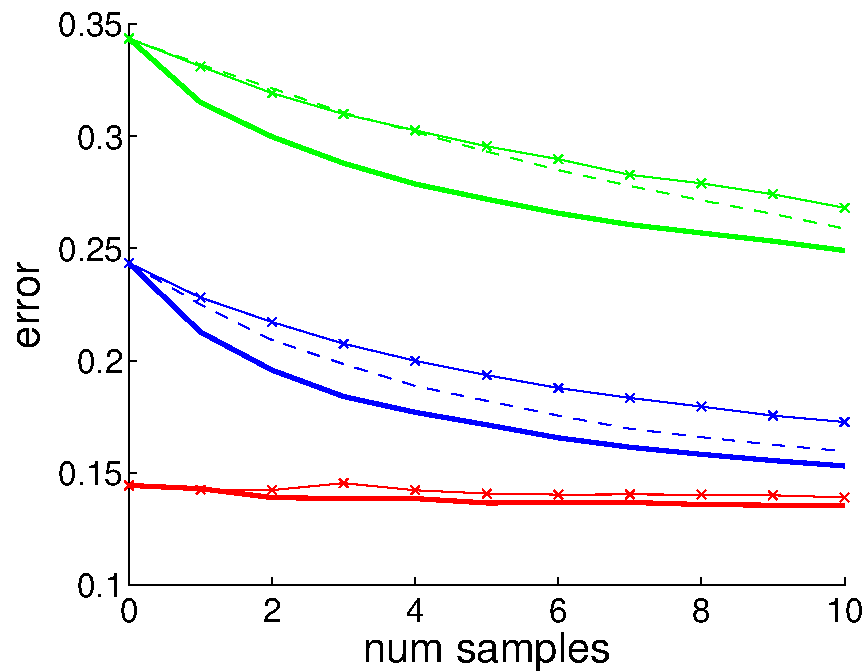
\includegraphics[scale=0.3]{figs/error_syntheticDataLargeScale.pdf}&
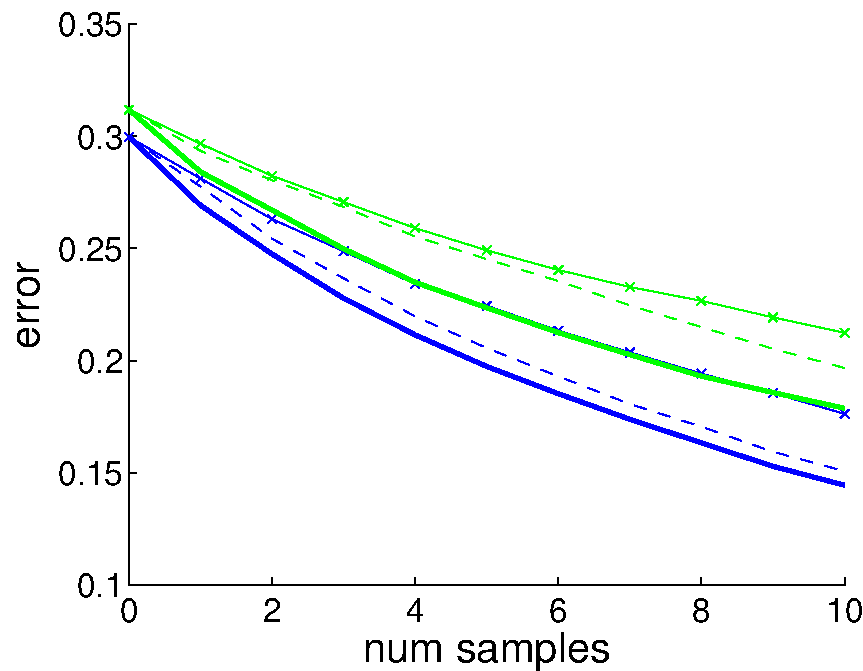
\includegraphics[scale=0.3]{figs/error_sushiDataLargeScale.pdf}&
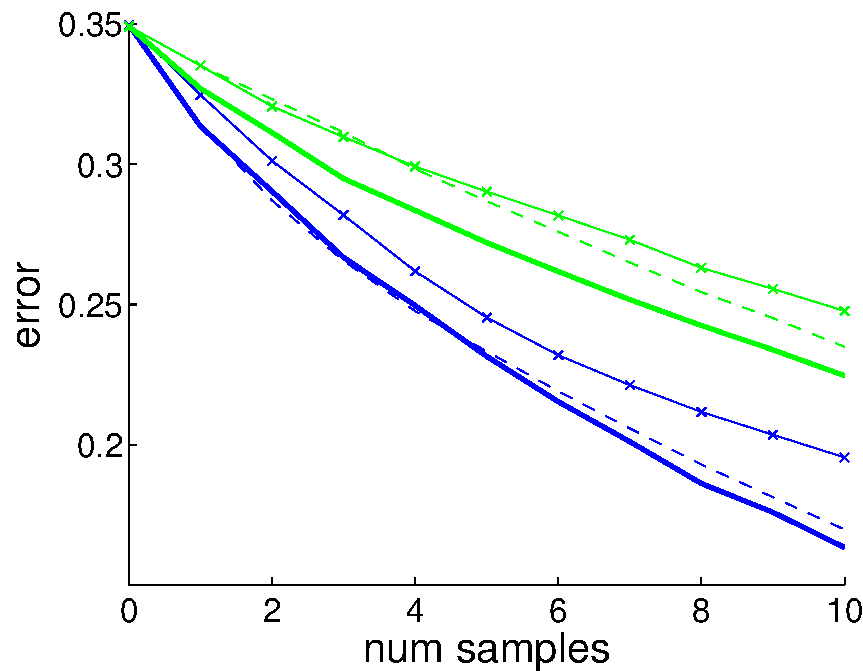
\includegraphics[scale=0.3]{figs/error_movieLensDataLargeScale.pdf}\\
Election&
Jura&
\\
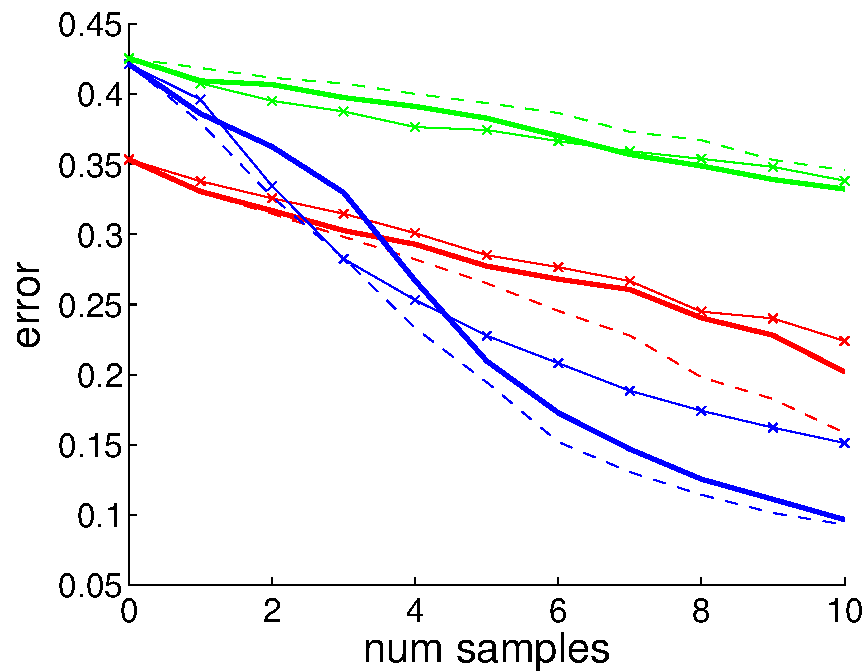
\includegraphics[scale=0.3]{figs/error_electionDataLargeScale.pdf}&
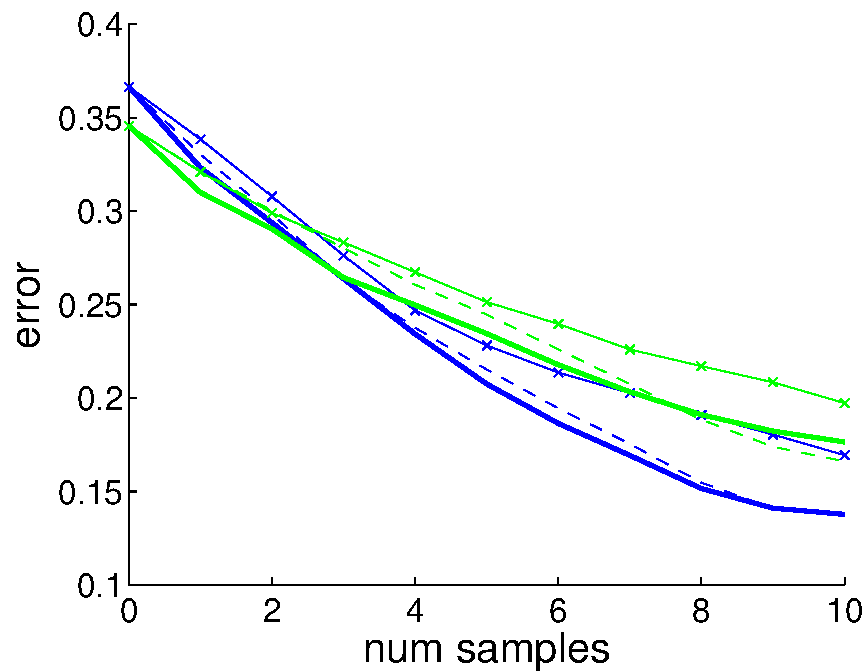
\includegraphics[scale=0.3]{figs/error_juraDataLargeScale.pdf}&
\hskip0.6cm \raisebox{0.08\height}{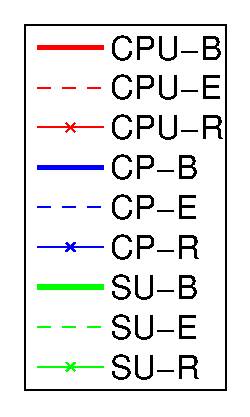
\includegraphics[scale=0.45]{figs/legend.pdf}}
\end{tabular}
}
\caption{Average test error for CPU, CP and SU, using the strategies BALD (-B), entropy (-E) and random (-R) for active learning.
For clarity, the curves for CPU are included only in the Synthetic and Election datasets.
The complete plots can be found in Section 10 of the supplementary material.\label{fig:learningcurves}}
\end{figure}

Here we evaluate the performance of BALD,
in particular, we compare CPU, CP, and SU using BALD (-B), Maximum Entropy Sampling (-E) and random sampling (-R).
We now use all the available users from each dataset, with a maximum of 1000 users.
For each user the available preference data are
split randomly into training, pool and test sets with 5, 35 and 5 data points respectively
in Synthetic, Sushi and MovieLens, 3, 22 and 3 data points in Election
and 3, 15 and 3 data points in Jura.
Each method is fitted using the training sets and its performance
is then evaluated on the corresponding test sets. After this,
the most informative data point is identified in each
of the pool sets. These data points are moved into the corresponding training sets
and the process repeats until 10 of these active
additions to the training sets have been completed.
The entire process, including the dataset splitting is repeated 25 times. 
Figure \ref{fig:learningcurves} shows the learning curve for each method.
For clarity, the curve for CPU is included only for the Synthetic and Election datasets; in the other datasets CPU is marginally outperformed by CP (see supplementary material, Section 10).
Average errors after 10 queries from the pool set of each user are summarized in Table \ref{tab:large}.
For each model (CPU, CP and SU), the results of the best active learning strategy are highlighted in bold.
The results of the best model/active learning strategy combination are underlined.
Highlighted results are statistically significant with respect to non-highlighted
results according to a paired $t$ test.
BALD always outperforms random sampling and usually outperforms or obtains equivalent performance to MES. 
In particular, BALD significantly outperforms MES in 9 cases,
while MES is better than BALD in only 2 cases.
